\documentclass[12pt,a4paper]{report}

% English
\usepackage[english]{babel} % English language setting
\usepackage[utf8]{inputenc} % Unicode text
\usepackage[T1]{fontenc} % German 'Umlaute'
\usepackage{textcomp} % Euro
\usepackage[hyphens]{url}
\usepackage{amssymb} % Symbols
\usepackage{emptypage} % Empty pages are now actually empty

% Fonts, with all the options
\usepackage{mathpazo}
\usepackage[scaled=.95]{helvet}
\usepackage{courier}
\usepackage{microtype}

% Images and listings
\usepackage{graphicx} % images
\usepackage{subfig} % sub-figures
\usepackage{wrapfig} % wrapping figures
\usepackage{listings} % better source code listings
\usepackage{enumitem}
\graphicspath{ {figures/} }

% Source code
\usepackage{float}
\newfloat{listing}{htbp}{scl}[chapter]
\floatname{listing}{Listing}
\usepackage{packages/coding/golang/lang} % import this package after listings
\usepackage{packages/coding/protobuf/lang}  % include language definition for protobuf
\usepackage{packages/coding/protobuf/style} % include custom style for protobuf declarations.
\lstset{
    basicstyle=\scriptsize\ttfamily,
    columns=[l]flexible,
    mathescape=true,
    showstringspaces=false,
    numbers=left,
    numberstyle=\tiny,
    frame=none,
    keywordstyle=\color{red},
    stringstyle=\color{blue},
    showstringspaces=false,
    tabsize=4,
    xleftmargin=\leftmargin,
    language=Golang
}

% Page layout
\usepackage[paper=a4paper,width=14cm,left=35mm,height=22cm]{geometry}
\usepackage{setspace}
\usepackage[htt]{hyphenat}
\usepackage{sectsty}
\linespread{1.5}
\subsubsectionfont{\large}

% Page markers
\newcommand{\phv}{\fontfamily{phv}\fontseries{m}\fontsize{10}{12}\selectfont}
\usepackage{fancyhdr} % nicer header and footer
\pagestyle{fancy}
\renewcommand{\chaptermark}[1]{\markboth{#1}{}}
\fancyhead[L]{\phv \nouppercase{\leftmark}}
\fancyhead[R]{\phv \thepage}
% rather not use anything for the footer
\fancyfoot[C]{\ } % no page count in the bottom
%\fancyfoot[R]{\textsf{\small Media Management}}

% Share the sources
\usepackage{bibtopic}

% Logo of the university
\usepackage{packages/hsrmlogo}

% Special packages
\usepackage{epigraph}
\setlength{\epigraphrule}{0pt} % no divider
\usepackage{csquotes}

% Some extra styles
\usepackage{soul}
\newcommand*\strikethrough{\st}

% Hyperlink everything
\usepackage{hyperref}
\hypersetup{
    bookmarks=true,
    colorlinks=true,
    linkcolor=black,
    citecolor=black,
    filecolor=black,
    urlcolor=black,
}
\urlstyle{same}

% Wikipedia-style "citation needed" macro
\newcommand{\cn}[1][]{\textsuperscript{\color{red} ~[citation needed]~}}

% Code markup
\newcommand{\code}[1]{\texttt{#1}}


\newcommand{\studyprogramme}{Media Management}
\newcommand{\degreetype}{Bachelor of Arts}
\newcommand{\thesistitle}{
The system and software architecture of back-end applications for the short-term rental of electric scooters
}
\newcommand{\thesissubtitle}{
Analysis of an existing legacy solution and evaluation of its extensibility
}
\newcommand{\thesisauthor}{Jakob Löhnertz}
\newcommand{\thesisdate}{23. Juli 2018}
\newcommand{\thesislocation}{Wiesbaden}
\newcommand{\firstmarker}{Prof.\ Dr.\ Johannes Luderschmidt}
\newcommand{\secondmarker}{Merle Hiort}

\begin{document}

\begin{titlepage}
  \begin{center}
    \hsrmlogo[1]
    \parbox[t]{8cm}{
      Hochschule \textbf{RheinMain}\\
      Fachbereich Design Informatik Medien\\
      Studiengang \studyprogramme}
    \\[1.5cm]
    {\LARGE Abschlussarbeit} \\[0.5cm]
    {\begin{spacing}{1} \large zur Erlangung des akademischen Grades \\[5mm] \end{spacing}}
    {\begin{spacing}{1} \large \degreetype \\[1cm] \end{spacing}}
    \rule{\textwidth}{1pt} \\[0.5cm]
    {\begin{spacing}{1.15} \huge \bfseries \thesistitle \\ \end{spacing}}
    {\begin{spacing}{1.15} \bfseries \thesissubtitle \\[0.60cm] \end{spacing}}
    \rule{\textwidth}{1pt}
    \\[1.5cm]
    \begin{tabular}{ll}
      Vorgelegt von & \thesisauthor \\
      am & \thesisdate \\
      Referent & \firstmarker \\
      Korreferent & \secondmarker
    \end{tabular}
  \end{center}
\end{titlepage}
\cleardoublepage

% Erklärung gemäß den Allgemeinen Bestimmungen für Prüfungsordnungen
\thispagestyle{empty}
\section*{Erklärung gemäß ABPO}
Ich erkläre hiermit, dass ich
\begin{itemize}
\item die vorliegende Abschlussarbeit selbstständig angefertigt,
\item keine anderen als die angegebenen Quellen benutzt,
\item die wörtlich oder dem Inhalt nach aus fremden Arbeiten entnommenen
  Stellen, bildlichen Darstellungen und dergleichen als solche genau
  kenntlich gemacht und
\item keine unerlaubte fremde Hilfe in Anspruch genommen habe.
\end{itemize}

\vspace{6em}
\noindent\begin{tabular}{p{0.37\textwidth}p{0.56\textwidth}}
\thesislocation, \thesisdate  & \rule{0.56\textwidth}{0.5pt}\\
              & \makebox[1cm]{\ } \thesisauthor
\end{tabular}

\vfill

\cleardoublepage



\begin{abstract}

The abstract will be added at this place towards the end of the thesis.

\end{abstract}


\tableofcontents



\chapter{Problems and research question} \label{chap:intro}

\epigraphhead[55]{\epigraph{Beauty is more important in computing than anywhere else
in technology because software is so complicated. Beauty is the ultimate defense against complexity.}
{\textit{David Gelernter}}}


The definition of the word \emph{scooter} is fairly vague.
Some describe it as a small vehicle with a handlebar and a platform to stand on,
the kind traditionally children were riding.
However, this paper looks at the \emph{motorcycle-esque type} of a scooter, and in
particular the electric version of it.

Many pain points of internal combustion engines vanish with the switch to their electric
counterparts. The maintenance of the mechanical system of the whole vehicle becomes easier.
There are less moving parts which makes for less errors.
On the downside, the exchange of the fuel causes the most problems with electric engines.
Of course they utilize batteries instead of fossil fuels as their impetus.
Although the invention of the battery is older than that of the
internal combustion engine\cn, the technology is still not perfected and sees new
advancements every year. Alas, it also combats many challenges in terms of
safety, cost, capacity, weight, recycling, speed of recharging and longevity.

For the provider, the handling of a short-term rental service
only becomes feasible with the automation of as many processes as possible.
This requires a back-end application ideally paired with a front-end.
Most of the time, ongoing human resource costs make up the biggest percentage
in the expenses of any business.\cn Thus, this demands for less human workforce
as part of the processes of a rental service.
Meanwhile, the upfront expenditures for the software development of
an application are still vast but in the long run, the running expenses are less.
The only cost driver afterwards is the maintenance of the created software.
As a consequence, the question should be how to mitigate the maintenance costs
of a software product. The main aspect is a proper application of
software engineering which is defined as:
\begin{displayquote}
\emph{"The application of a systematic, disciplined, quantifiable approach to the
development, operation, and maintenance of software."}~\cite{se-ieee}
\end{displayquote}
To put this definition into words, software engineering mainly targets
the domains of software architecture, code quality and documentation.\cn\\
All of these pursue one long-term goal: to achieve a well functioning, maintainable
software product.

Furthermore, the fact that the scooters are always connected to the internet
as well as the nature of current batteries desire a reactive and faultless application.

Finally, the corporate partner of this thesis, which is discussed in detail
in section \ref{sect:kumpan}, is already in possession of a solution which is not fully featured yet.
Therefore, the subject of extending an existing back-end application with missing features is also targeted.

In conclusion, this leads into the research question of this bachelor thesis:\\
\emph{Which functional modules are necessary for the implementation of a back-end application
for the short-term rental of electric scooters and which considerations need to be made
to integrate additional functionality into an existing legacy software solution for that purpose?}



\chapter{Fundamentals} \label{chap:fundamentals}

\epigraphhead[55]{\epigraph{The danger in the sequence [waterfall approach]
is that the project moves from being grand to being grandiose,
and exceeds our human intellectual capabilities for management and control.}
{\textit{Harlan D. Mills}}}


\section{The market for the rental of electric scooters}

The market for the short-term rental of motor vehicles in Germany
is currently growing rapidly~\cite{bundesverband-carsharing-statistics}.
The situation on the market is no different for medium and long-term rentals~\cite{sparkasse-kfz-vermietung}.
However, this sector is dominated by cutthroat competition.
It has been dictated by large corporations such as \textit{Sixt}, \textit{Hertz},
\textit{Avis} and \textit{Europcar} for years~\cite{sparkasse-kfz-vermietung}.
Although smaller providers exist, this market has become an oligopoly and
the barriers for a market entry are high for new types of providers.

In contrast, the market for short-term rental, also known as car sharing for cars,
is a comparatively young market. It has only existed in Europe in its breadth
since the late 1980s~\cite{history-of-carsharing} and in its current form
only since the advent of the smartphone, since many offers require the use of a mobile app.
For this reason the market for short-term rentals and thus its saturation is significantly lower.
According to the \textit{Bundesverband CarSharing e.V.}, the current total number of cars
in the car sharing sector in Germany is about 17,200. In contrast, almost 10\% of all
new vehicle registrations in Germany in 2015 were attributable to traditional
car rental companies such as the above~\cite{sparkasse-kfz-vermietung}.
This represents an increase of 339,000 vehicles, in similar fashion every year.
By contrast, the share of vehicles with electric drive is again lower at
just under 10\% of the total number of car sharing vehicles.
Electric scooters do not even appear in the statistics of the
\textit{Bundesverband CarSharing e.V.}~\cite{bundesverband-carsharing-statistics}.

However, the market in other nations has already experienced strong growth;
one example is the Chinese market. Around 20 million electric scooters were sold
there in 2016 alone~\cite{heise-electric-scooters}.
Additionally, the short-term rental of these is already a working business model
in China~\cite{allchinatech-electric-scooters}. Market value forecasts are also promising.
Last year, the US company \textit{P\&S Market Research} predicted an annual growth of
just under 7\% in the market for motorized two-wheeled vehicles with
electric drive until 2025~\cite{pands-electric-scooters}.
The totality of these figures and the status quo in China create a positive impression
with regard to the possibility of a successful market entry into this sector in Germany.
The future of the market is also promising, as more and more nations around the world
are deciding on a ban on vehicles with internal combustion engines for the
foreseeable future~\cite{faz-combustion-engine-ban} and companies already
in the market are undertaking their first expansions~\cite{allchinatech-electric-scooters, faz-electric-scooters}.


\subsection{German electric scooter manufacturer \textit{Kumpan}} \label{sect:kumpan}

The thesis loosely focuses on the business of German electric scooter manufacturer \textit{Kumpan}.
The company was established in 2009. For their product, they concentrated on three main aspects:
an exterior design ready for the European market, build quality and sufficient cruising radius.
They finished building their first electric scooter in 2010 and are thriving for good products ever since.
The price of their electric scooters is still rather high. Owing to that circumstance,
they came up with smaller, cheaper models as well as a completely different approach.

Instead of traditional retail sales they started developing the idea of a
short-term rental service for their scooters. And from many angles it makes sense:
As seen in the last section, the market for the short-term rental of electric scooters
especially in Germany is still minuscule compared to e.g. car or bike sharing.
Meanwhile, the costs for buying an electric scooter are still relatively high.
Additionally, many people will not need such a vehicle for the whole day and would benefit
from more flexibility. Lastly, parking spots are also a scarcity in inner cities.
Therefore, \textit{Kumpan} plans to enter the market of short-term electric scooter rentals
in the near future.

There are still many aspects to be discussed and determined but one of them
is already set and can be seen as a necessity regardless of the final implementation:
A server back-end application as well as its infrastructure.
\textit{Kumpan} purchased an existing software solution to achieve this.
Beforehand, it was already known though that the software is not feature-complete
for their usage. Thence, it is already planned to extend the software with the missing
features.


\section{Components of a modern software product}

The main aspect of success for such a system is indeed the \emph{magic} behind the scenes
that no customer sees. People just see the electric scooter as the product and
want to be able to ride one on demand by just pushing a button.
The ease of use for the customers and their satisfaction are the main facets
to be considered by the provider of such a service.

This, as nearly every modern software product geared towards a general audience,
involves two foundational components --- a front-end and a back-end~\cite{fischer-lexikon}.
On the one hand, the front-end provides the user interface of the product, the façade of the whole.
It is the component the customer interacts with but more importantly it will be
what the users identify the product with.
On the other hand, the back-end is the brain of the software product.
It provides endpoints for the front-end to use and consume. The back-end dictates
what the front-end will do. Meanwhile, it does not determine what it will look like.
If the front-end is unusable the back-end will never be able to fix that as the
front-end becomes the mental representation of the whole product for the customers.
If the back-end behaves sluggish or is prone to errors, the front-end will not be able to save much
by the same token. In the end, both form a synergy with each other.

This thesis will shed light on the back-end of such an application.
It will focus on the software architecture of it.
This includes the functionalities that are mandatory and the question on how the product
might come together; from ideas and drafts to written source code.


\subsection{Necessity of a thorough back-end application}

A look at existing car sharing offers depicts that automating the rental process
is necessary. There are three main aspects that become easier to achieve for the
provider if they choose to automate their system.\\
Firstly, as already mentioned in the first chapter,
the costs are a lot lower whenever less human resources are involved.
Additionally, the speed of execution of a rental request by a customer gets better
with a performant back-end application.
Finally, a modern software solution attracts more customers as the ease of use
is expected to be better. Furthermore, the entrance barrier to try a rental service
gets lower. Nowadays, customers, especially younger ones, are used to web-based
or mobile app-based software and are a lot more likely to try out such an offer.~\cn
Although, the users are never in contact with the back-end, it is absolutely
crucial for the success of the whole application as the front-end just displays
the information in a presentable way while not performing any serious
business logic most of the time.


\section{Approaching the development of software} \label{sect:software-development-process}

From a very fundamental standpoint, software development consists of two distinct phases.
The planning and analysis phase which leads into the programming phase~\cite{royce-large-systems}.
Upon further investigation, there are more steps before, in between and after these two essential ones.
In his influential 1970 paper \textit{"Managing the Development of Large Software Systems"},
American computer scientist Winston W. Royce discusses his idea of a satisfactory
software development process. His paper is often mistakenly cited as the starting point
of the \textit{waterfall model} whereas Royce indeed starts his paper with such an approach but quickly
depicts the shortcomings of that model~\cite{royce-large-systems, larman-iid-history}.
The waterfall model describes the idea that a software development process should consist of
the stages shown in figure \ref{fig:waterfall-model}.
\begin{figure}[htb]
\centering
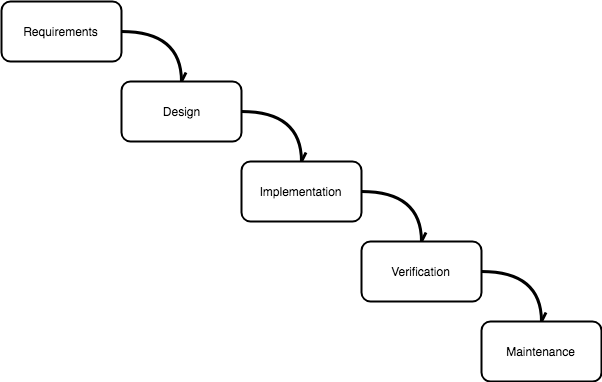
\includegraphics[width=.60\textwidth]{waterfall-model}
\caption{The essential stages of the waterfall model}
\label{fig:waterfall-model}
\end{figure}
The main point of it is that the steps are conducted sequentially; no step should
begin before the current one has been finished~\cite{boehm-spiral}.
This idea has one big flaw: the \textit{Verification} phase being nearly at the end.
Only after the whole software product is finished, an evaluation by internal testing personnel or
the client can be carried out~\cite{royce-large-systems}.
It is likely that at least some changes to the implementation will be necessary after the \textit{Verification}.
Additionally, clients may not know the exact requirements at the very beginning
of the software development process~\cite{parnas-rational-design-process}.
It is also possible that a major fault is only discovered in that second last stage ---
the negative repercussions could be massive.
\begin{displayquote}
\emph{"Either the requirements must be modified, or a substantial change
in the design is required. In effect the development process has returned to
the origin and one can expect up to a 100-percent overrun
in schedule and/or costs."}~\cite{royce-large-systems}
\end{displayquote}
Nevertheless, the idea Royce describes is what made his paper as influential.
The steps that are required to get from an idea to a finished product nearly always
stay the same. The ones from figure \ref{fig:waterfall-model} are still applicable to
many newer concepts of a software development process.

Nowadays, software developers and project managers are mostly utilizing any model that
can be subsumed under the loose term \textit{agile}.
In summary, as the term already depicts, this theory is geared towards
the idea that the software development process should not be as rigid and constrained.
Therefore, it stands in stark contrast to the demonstrated waterfall model.
The term does not describe a distinct concept but rather an idea ---
there are dozens of implementations of agile software development~\cite{martin-agile-practices}.
Regardless of the implementation, most often agile approaches are based around
the idea of \textit{Iterative and Incremental Development (IID)}~\cite{larman-iid-history}.
\begin{displayquote}
\emph{"Software development should be done incrementally, in stages with
continuous user participation and replanning and
with design-to-cost programming within each stage."}~\cite{mills-iid}
\end{displayquote}
\newpage
Instead of implementing the whole software within all the sequential steps
of the waterfall model, the product is being developed in increments.
Following some initial analyzing and planning, the first iteration begins.
After the end of one iteration of all the steps shown, apart from the \textit{Maintenance},
the next increment is getting projected and eventually executed as shown in figure \ref{fig:idd-model}.
\begin{figure}[htb]
\centering
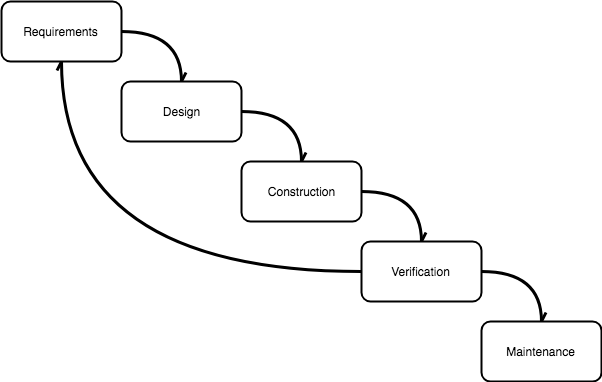
\includegraphics[width=.60\textwidth]{iterative-and-incremental-model}
\caption{A revised, iterative version of the waterfall model e.g. IID}
\label{fig:idd-model}
\end{figure}\newline
To conclude, the stages Royce exhibited in 1970 are still applicable nowadays.
In some form or another, those are mandatory for implementing any software.
In the following subsections, the portrayed stages are discussed in greater detail,
while excluding the last two ones as they will not be part of the \textit{Analysis}-chapter \ref{chap:analysis}.


\subsection{Requirements}

\subsection{Design}

\subsection{Implementation}


\section{Legacy software} \label{sect:legacy-software}

The term \textit{legacy software} describes a software product that was created
some time in the past and thus became outdated in terms of the utilized technology
stack, its performance and security or its software architecture~\cite{seacord-modernizing-legacy}.
All of the above can occur at once or emerge partially.\\
The term often bears a pejorative association with it although legacy software
is still indispensable for the organization that makes use of it. Most of the time, it
still fulfills the needs of its users and is therefore still profitable~\cite{bennett-coping-legacy}.
Moreover, the source code sometimes comprises the knowledge of the organization while
the software itself is archaic. Owing to that fact, discontinuing legacy software can be difficult.
Additionally, on the one hand, many problems arise with the operation of legacy systems but,
on the other hand, there are also compelling reasons for an organization
to keep a legacy system running. Both of these facets are discussed in the following sections.
In the end, there are two general options: a complete replacement of the legacy system or
a partial extension of it.


\subsection{Reasons to continue legacy software} \label{sub-sect:continue-legacy}

Formerly, a main reason to keep a software solution running was tied to its
hardware requirements. Legacy software that is many decades old might still
run on mainframe computers opposed to contemporary server systems~\cite{schneidewind-preserve-or-redesign}
or even cloud computing. However, these considerations are not part of this thesis
since the analyzed software solution was built as a common client-server application
meant to run on prevailing server infrastructure.

Apart from this initial reason, the most common one is of economic nature~\cite{schneidewind-preserve-or-redesign}.
Often times, the expected benefits of redeveloping a software cannot justify the expenditures.
Additionally, it is difficult to measure the advantages beforehand. The management
of a company needs to ponder the proposal of redeveloping the current software.
Particularly, if the legacy software still seems to be running as expected when observed
from the outside, is becomes harder for the developers and engineers to vindicate
their proposal towards the management --- raw characteristics such as performance,
security, maintainability and eventually the development time can just be roughly estimated and
are bound to the experience of the developers and engineers in charge.
Moreover, even if the analysis does sound promising there is no guarantee that the new system
will meet the expectations. Nevertheless, the tipping point can occur when the human costs for the maintenance
of the legacy software are tremendous when compared to development teams of similar size and complexity.

Furthermore, required constant availability or faultlessness of a system might make it
difficult or impossible to implement a new software solution for its purpose~\cn ---
software that controls a nuclear power plant comes to mind, for instance.
Economic considerations offer an additional point of view:
\begin{displayquote}
\emph{"If a legacy system is running the key billing system, it is not sensible
to make rash judgments, because the very future of the business may be at stake."}~\cite{bennett-coping-legacy}
\end{displayquote}
Especially the testing of a critical application might increase the costs
and/or risks significantly. These aspects might make it improbable to replace
the legacy software. Owing to the fact that the legacy software still fulfills
its purpose, much effort is needed to ensure that the replacement software works
in the same expected and quantifiable manner as its legacy counterpart.

In addition, it is also possible that the users of the legacy software do not want
to switch to a new solution due to third-party vendor lock-in or the fact that
they are familiar with the legacy system~\cite{bennett-coping-legacy} which would make
retraining a vast cost driver.

Lastly, a big concern that the company's management cannot even control is
poor or missing documentation.~\cn This circumstance is the most difficult one
as it makes the redevelopment or the extension of the legacy software very intricate.
Consequently, this can go as far to leave the organization unable to completely apprehend
every detail of its legacy software.

In summary, these four aspects are mostly accountable for the continuation of legacy software
within an organization. Albeit, the assessment of costs versus benefits
can be seen as the most important one by far~\cite{schneidewind-preserve-or-redesign}.


\subsection{Issues with legacy software} \label{issues-legacy-software}

The last-named reason of a poor documentation in favor of continuing a
legacy system is likewise a major issue~\cite{bisbal-legacy-issues}.
The developers know far less about potential side-effects and thus
fixing a bug or refactoring some source code becomes a tedious task.
In consequence, human expenditures escalate compared to a well-known and well-documented
solution owing to the fact that any activity on the legacy system takes more time.
After all, the maintenance of poorly documented legacy software
is more time-consuming and thus more costly.

The second issue emerges when a legacy software solution receives many
patches and general improvements over time; its maintenance
turns into a problem. The system becomes overly brittle due to its
increasing complexity~\cite{seacord-modernizing-legacy, tilley-perspectives-reengineering}.
This brittleness engenders a growing number of side-effects and bugs
to the point where further extending the software becomes an ordeal.

The final issue is about the absence of proper interfaces
in legacy systems~\cite{bisbal-legacy-issues}. This problem manifests itself twofold.
Firstly, integrating a legacy system into another system is onerous.
Legacy software often completely lacks an externally accessible API.
Therefore, connecting an aged technology stack of a legacy system to a completely
different type of architectural design, most often running on a different programming language,
might be virtually impossible or only achievable with severe wrapping
of the interfaces of the legacy system. However, that intensifies the aforementioned
issue of high human costs all the more.
Secondly, the extensibility of a legacy system is worse.
The developers that once created the legacy software might not be part of the
organization anymore. If this fact is paired with poor documentation and/or
an inferior software architecture, extending such a legacy solution is once again
very time-consuming. For example, if a legacy software features
low cohesion but high coupling, the converse way of how it should be~\cn,
extending it might introduce unwanted side-effects which increase debugging
time by a large margin.


\subsection{Solutions to legacy software issues}

Although, as just mentioned, the extensibility of legacy software might be mediocre,
a couple of concepts do exist to overhaul an existing legacy software solution.
Generally speaking, they range from an evolution to a revolution~\cite{bisbal-legacy-issues}.
The approach of \textit{Maintenance} is excluded from this subsection as it
has to be applied to every software product as shown in section \ref{sect:software-development-process}.
Nevertheless, it is a legitimate approach to cope with legacy software.
In consequence, four main concepts can be defined as solutions to legacy software issues ---
they are displayed in the following figure \ref{fig:coping-legacy}.
The axis depicts the amount of changes each approach entails.
However, it is important to discern that it is likely that a combination of
the explained concepts is utilized~\cite{bisbal-legacy-issues}.
Some parts of a legacy system might be wrapped while others need to be redeveloped.
\begin{figure}[htb]
\centering
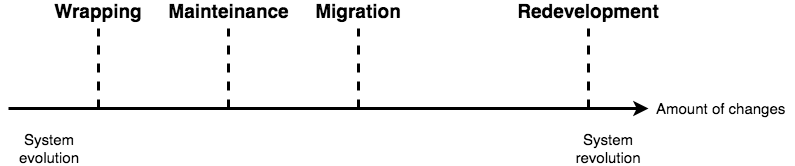
\includegraphics[width=.80\textwidth]{coping-with-legacy-systems}
\caption{Four approaches to cope with legacy software systems~\cite{bisbal-legacy-issues}}
\label{fig:coping-legacy}
\end{figure}


\subsubsection{Redevelopment}

To start from the far right, \textit{Redevelopment} is the most disruptive approach;
it implicates the discontinuation of the currently used software.
While having the huge disadvantage of being immensely cost-intensive, it indisputably
yields the best results opposed to the issues with legacy software presented in
subsection \ref{issues-legacy-software}.
Nevertheless, the second big risk apart from economic concerns is
the risk of failure.
Finally, depending on the size of the project, it is possible that at the end
of a long development cycle for the new software solution, it becomes outdated
yet again by not fully meeting the ever-changing
business needs anymore~\cite{stevens-software-reengineering-patterns}.


\subsubsection{Migration}

A median concept on the scale of figure \ref{fig:coping-legacy} is \textit{Migration}
which is also known as \textit{Reengineering}~\cite{tilley-perspectives-reengineering}.
These hypernyms actually describe two different solutions in terms of their goals;
they are, however, often used interchangeably~\cite{bisbal-legacy-issues}.
While both terms imply the extension of a legacy system, \textit{Reengineering}
has the goal to phase out the existing system eventually.
On the other hand, \textit{Migration} is just about augmenting the currently used
solution with new functional components while replacing some others that cannot be used anymore
for any reason. To put it into the words of Jesús Bisbal et al.:
\begin{displayquote}
\emph{"Migration seeks to reuse as much of the legacy information system as possible,
including implementation, design, specification, and requirements."}~\cite{bisbal-legacy-issues}
\end{displayquote}
Meanwhile, Scott R. Tilley and Dennis Smith define \textit{Reengineering} as:
\begin{displayquote}
\emph{"Reengineering is the systematic transformation of an existing system
into a new form […]"}~\cite{tilley-perspectives-reengineering}
\end{displayquote}
Consequently, these definitions put \textit{Reengineering} closer to \textit{Redevelopment},
due to the fact that both pursue the same long-term goal.
Nevertheless, in their execution, \textit{Migration} and \textit{Reengineering}
are conducted similarly.\\
Concretely, there are four major approaches to a \textit{Migration}
process~\cite{malinova-legacy-techniques}, ranging from a moderate one
to the just mentioned \textit{Reengineering} which is oftentimes a larger proposition.

\paragraph{Retargeting}
If for any reason the hardware or utilized third-party software got outdated,
the legacy software can be migrated to more performant hardware or
up-to-date versions of the leveraged third-party software.\\
\textit{Example}: Migrating the existing legacy software from traditional server
hardware to cloud-computing.

\paragraph{Conversion}
However, the changes in hardware or third-party software might be too disruptive
to perform them directly. In that case, a \textit{Conversion} of utilized
programming languages or technology stacks can be conducted.
Of course, this process is accompanied by much more work.\\
\textit{Example}: Converting the existing non-relational database to a
new database management system (DBMS) which is based on the relational SQL.

\paragraph{COTS components}
Furthermore, \textit{commercial-off-the-shelf (COTS) components} can be
leveraged to replace certain parts of a legacy software solution which oftentimes also
augments it, owing to the fact that such products are usually offering a wide
variety of features.\\
\textit{Example}: Replacing the customer management component of an existing
legacy software with a current COTS customer \textit{customer relationship management (CRM)} solution.


\subsubsection{Wrapping}

To conclude, \textit{Wrapping} is the least revolutionary process.
In fact, it actively endorses the continuation of a legacy software solution as
portrayed in subsection \ref{sub-sect:continue-legacy}.
This concept involves wrapping the existing codebase into an isolated package
which is then just accessed via a newly created interface e.g. an API.
The existing legacy software receives input parameters and returns an output.
The substantial problem with this whole concept is that the legacy software does get
extended only unidirectionally. It cannot invoke calls towards the newly added components.
Therefore, this solution is rather short-term in nature.
This concept can be divided into four distinct levels~\cite{sneed-encapsulating-legacy}.

\paragraph{Database}
A \textit{database wrapper} is the least interfering approach due to the fact that
the existing source code can stay as it is; it just exposes the database of the current system
to the outside.\\
\textit{Example}: The database table persisting the print jobs of an existing legacy software
is available for external programs.

\paragraph{Service}
The \textit{service wrapper} encapsulates distinct services from the legacy software
into callable entities which can thus be invoked from an external system.\\
\textit{Example}: The entire reservation system of an existing legacy software
can be called via an API by an external system.

\paragraph{Application}
An \textit{application wrapper} provides single classes or whole components for external usage.
It is similar to a \textit{service wrapper}, however, the wrapping is applied on a more
compartmentalized level.\\
\textit{Example}: The object of a class to create print jobs in a certain format
gets exposed to the outside, allowing it to be used by external programs.

\paragraph{Function}
Finally, \textit{function wrappers} attach to the most microscopic portions of a software ---
its functions. This approach can be useful if both low cohesion and low coupling are prevalent
in the present legacy software.\\
\textit{Example}: A single function that calculates a specific taxation value
can be invoked by an external process.
\newline

To sum up, Robert C. Seacord also mentions \textit{Black-Box Modernization} as well as
\textit{White-Box Modernization}~\cite{seacord-modernizing-legacy} which are
effectively \textit{Wrapping} and \textit{Migration}. To put this into words,
if an organization conducts the \textit{Wrapping} approach, the main goal is not
to handle the internals of the legacy software.
Meanwhile, a \textit{Migration} process embraces subtle changes to the codebase of the software.\\
In consequence, owing to the fact that most of the time \textit{Wrapping} still
involves some changes to the codebase, \textit{Migration} can be a better
approach since it results in a longer-term solution.\\
Nevertheless, the primary focus of both approaches is to achieve a greater
return on investment (ROI) compared to a \textit{Redevelopment}~\cite{tilley-perspectives-reengineering}.



\chapter{Analysis} \label{chap:analysis}

\chapter{Implementation} \label{chap:implementation}

\chapter{Conclusion} \label{chap:conclusion}



\newpage

% Source lists
\listoffigures
% \listoftables
\newpage

% Separate the sources with 'bibtopic'
\bibliographystyle{plain}
\begin{btSect}{offline}
\section*{References}
\btPrintCited
\end{btSect}
\begin{btSect}{online}
\section*{Online Sources}
\btPrintCited
\end{btSect}

\end{document}
